\chapter{Introduction}
\label{intro} % Always give a unique label

% \epigraph{``All children are artists. The problem is how to remain an artist once he grows up."(This is not necessary if you don't want it.)}
% {Pablo Picasso}

% \section{Introduction}
% \label{sec:Introduction}
\section{Problem Formulation}
Many interventional procedures rely on needle insertion, including biopsy and brachytherapy. Accurate needle placement is a critical factor in the success of these procedures. Deflection of the needle tip during insertion and variation in the mechanical properties of tissue cause the needle to deviate from its expected trajectory and miss the target. A common strategy to mitigate this is to use an alignment structure to aim the needle at the target and to verify that the correct position has been reached in post-operative imaging. Even with these techniques several insertions may be required to successfully reach the target.

Live intra-operative imaging of the needle throughout insertion mitigates error caused by needle deflection by allowing the surgeon to see if the needle is deviating from its trajectory and take action to correct. Ultrasound and Magnetic Resonance Imaging (MRI) are common imaging modalities. Manually-controlled image-guided needle insertion is still a challenging task: when using US imaging the surgeon must control both the needle and the transducer, while the confined space of the MRI scanner bore limits the surgeon's visibility and range of motion.

Robotically-controlled needle insertion using intra-operative imaging can correct for unmodeled tip deflection and keep the needle on its expected trajectory, improving the success rates of biopsies and other needle-based interventions. Several collaborative needle insertion robots have been demonstrated, where the surgeon controls the rate of needle insertion and the robot controls needle orientation.


*** Problem formulation: A key requirement in robotic image-guided needle insertion is the localization of the needle tip in each image and the calculation of the needle tip pose. Observation of the needle tip during insertion is required. Prior work in needle tip localization has generally searched for the needle in each image separately, but this is inaccurate in scenarios where significant noise or other needle-like shapes are present. Fully-autonomous needle tip tracking in clinically-representative situations is very challenging.


Previous work such as \cite{AIMNeedleSteering} has shown that closed-loop control of MRI scan planes coupled with image processing techniques for needle localization can track a needle tip during insertion with a useful degree of accuracy.

\subsection{Needle Artifact}
Needle artifact is caused by distortion of magnetic field by metal needle. Shape of artifact depends on material, orientation, scan plane parameters, imaging strategy.

\subsection{3D Slicer}
3D Slicer\cite{Fedorov2012Slicer} is an open-source GUI-centered tool for performing medical image processing and image-guided procedures. It provides a common standard and familiar interface for medical researchers, and lots of new imaging research is released as Slicer modules.

\subsection{OpenIGTLink}
OpenIGTLink is a communication standard for image-guided therapy (IGT) that supports sending and receiving images, DICOM data, and 3D homogeneous transforms between devices and programs via TCP/IP. 3D Slicer includes an OpenIGTLink extension to allow communication with imaging devices like MRI and ultrasound and control of robotic surgical tools.

\section{Thesis Contributions}
- What does this work do that's new? What's most important?

* Model-based needle tip pose estimation

** Use of real-time kinematic info from insertion robot

* Slicer modules

* 3D needle tip tracking using real-time data

*** Key contribution: Including the forward kinematics of the insertion robot and the mechanical properties of the needle enhances localization of the needle tip by limiting the search area, reducing the required frequency of new images, and reducing the likelihood that the imaging process will lose tracking of the needle tip during insertion. This is implemented as a parametric polynomial curve fit to intersect detected needle points while minimizing the bending energy in the needle.


A robotic needle insertion system provides kinematic data which can be used to calculate the pose of the needle base in the global frame. In combination with a mechanical simulation of needle deflection throughout insertion, the pose of the needle tip can be found in the global frame. The modeled needle tip pose can be used during real-time insertion tracking to plan imaging. The expected result is that the tip pose of a needle can be estimated to some comparatively high degree of accuracy throughout a live insertion, which could be used for needle trajectory control and error compensation.







% This is the Literature Review Section. Here is a figure: Fig.\ref{fig:exampleFigure} and here is a table: Table \ref{tab:Protocol}.

% \begin{figure}[h]
%   \begin{center}
%     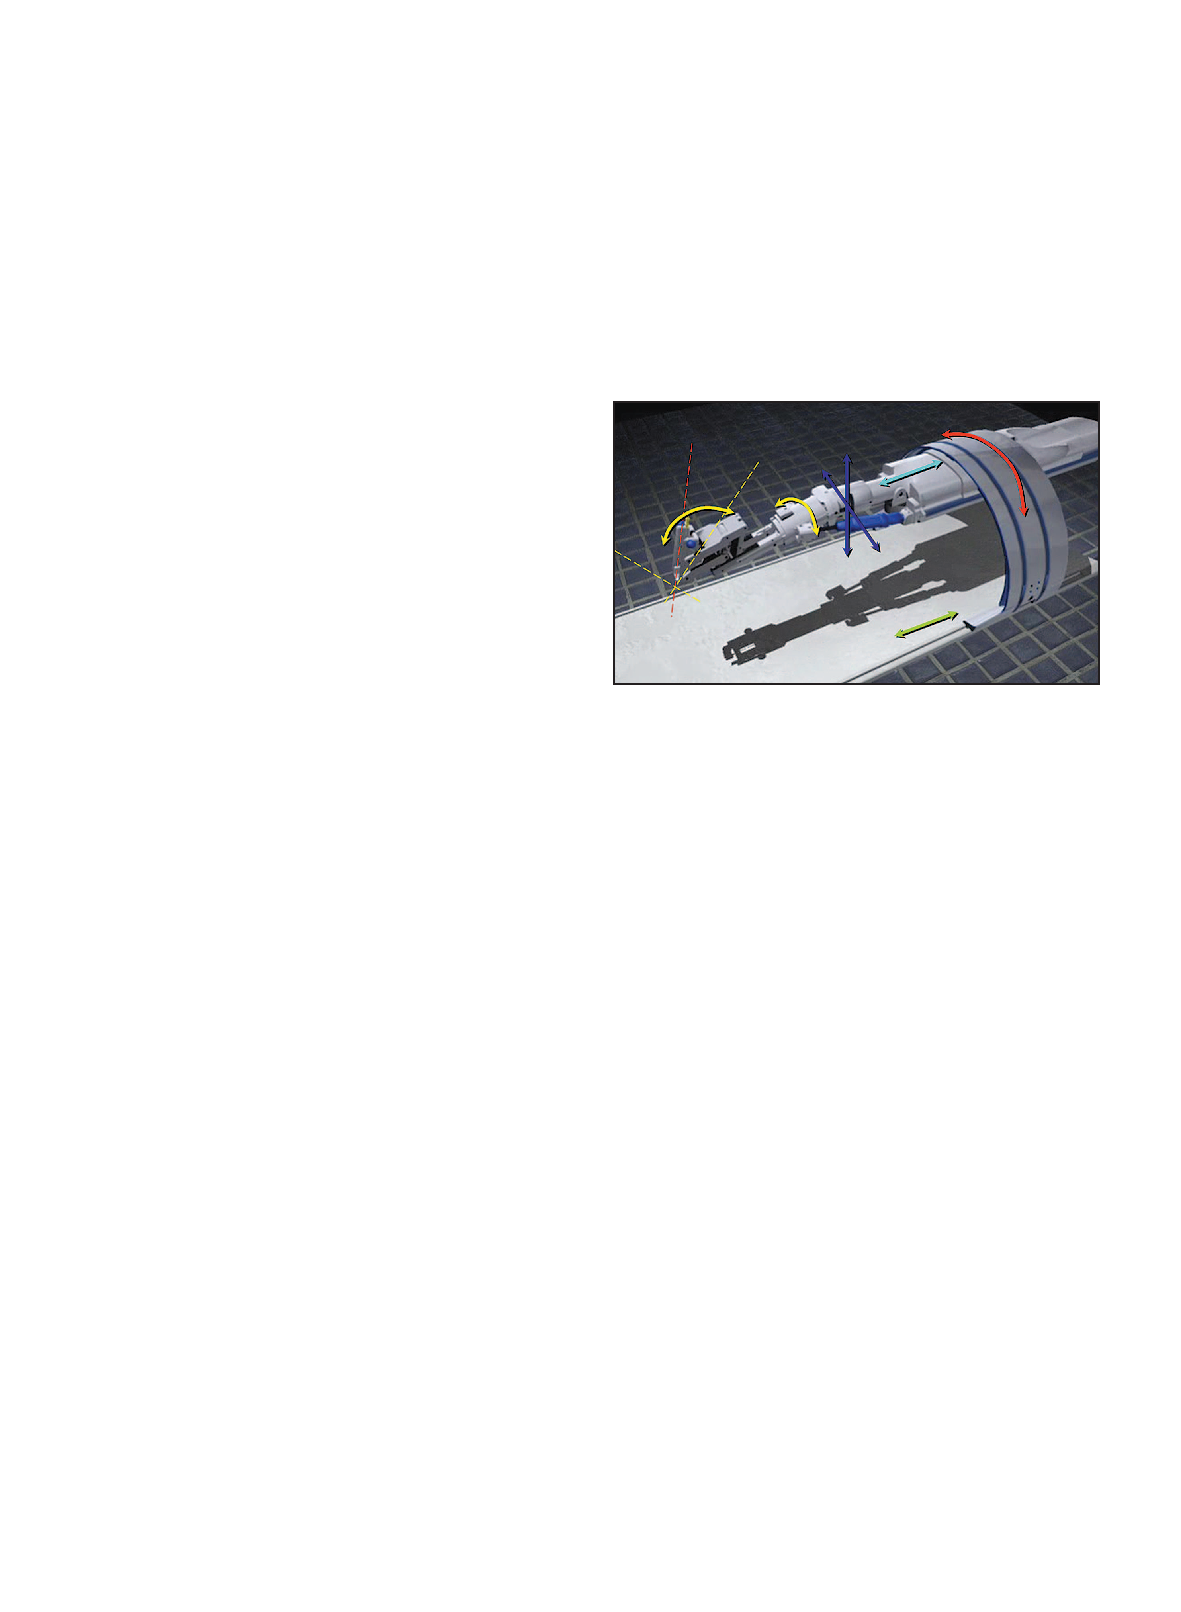
\includegraphics[width=120mm]{Fig/chap1/innomotion.pdf}
%   \end{center}
%   \vspace{-4mm}
% \caption[CAD model of the Innomotion robotic system.]
% {This is a sample figure with a sample citation \cite{Fischer2008_TMECH} \copyright 2008 IEEE.}
%  \label{fig:exampleFigure}
% \vspace{-2mm}
% \end{figure}

% \begin{table}[htb]
%   \begin{center}
% \caption[Scan parameters for compatibility evaluation.]{Detailed scan parameters for each of four protocols for compatibility evaluation}
% \label{tab:Protocol}
%   \end{center}
% 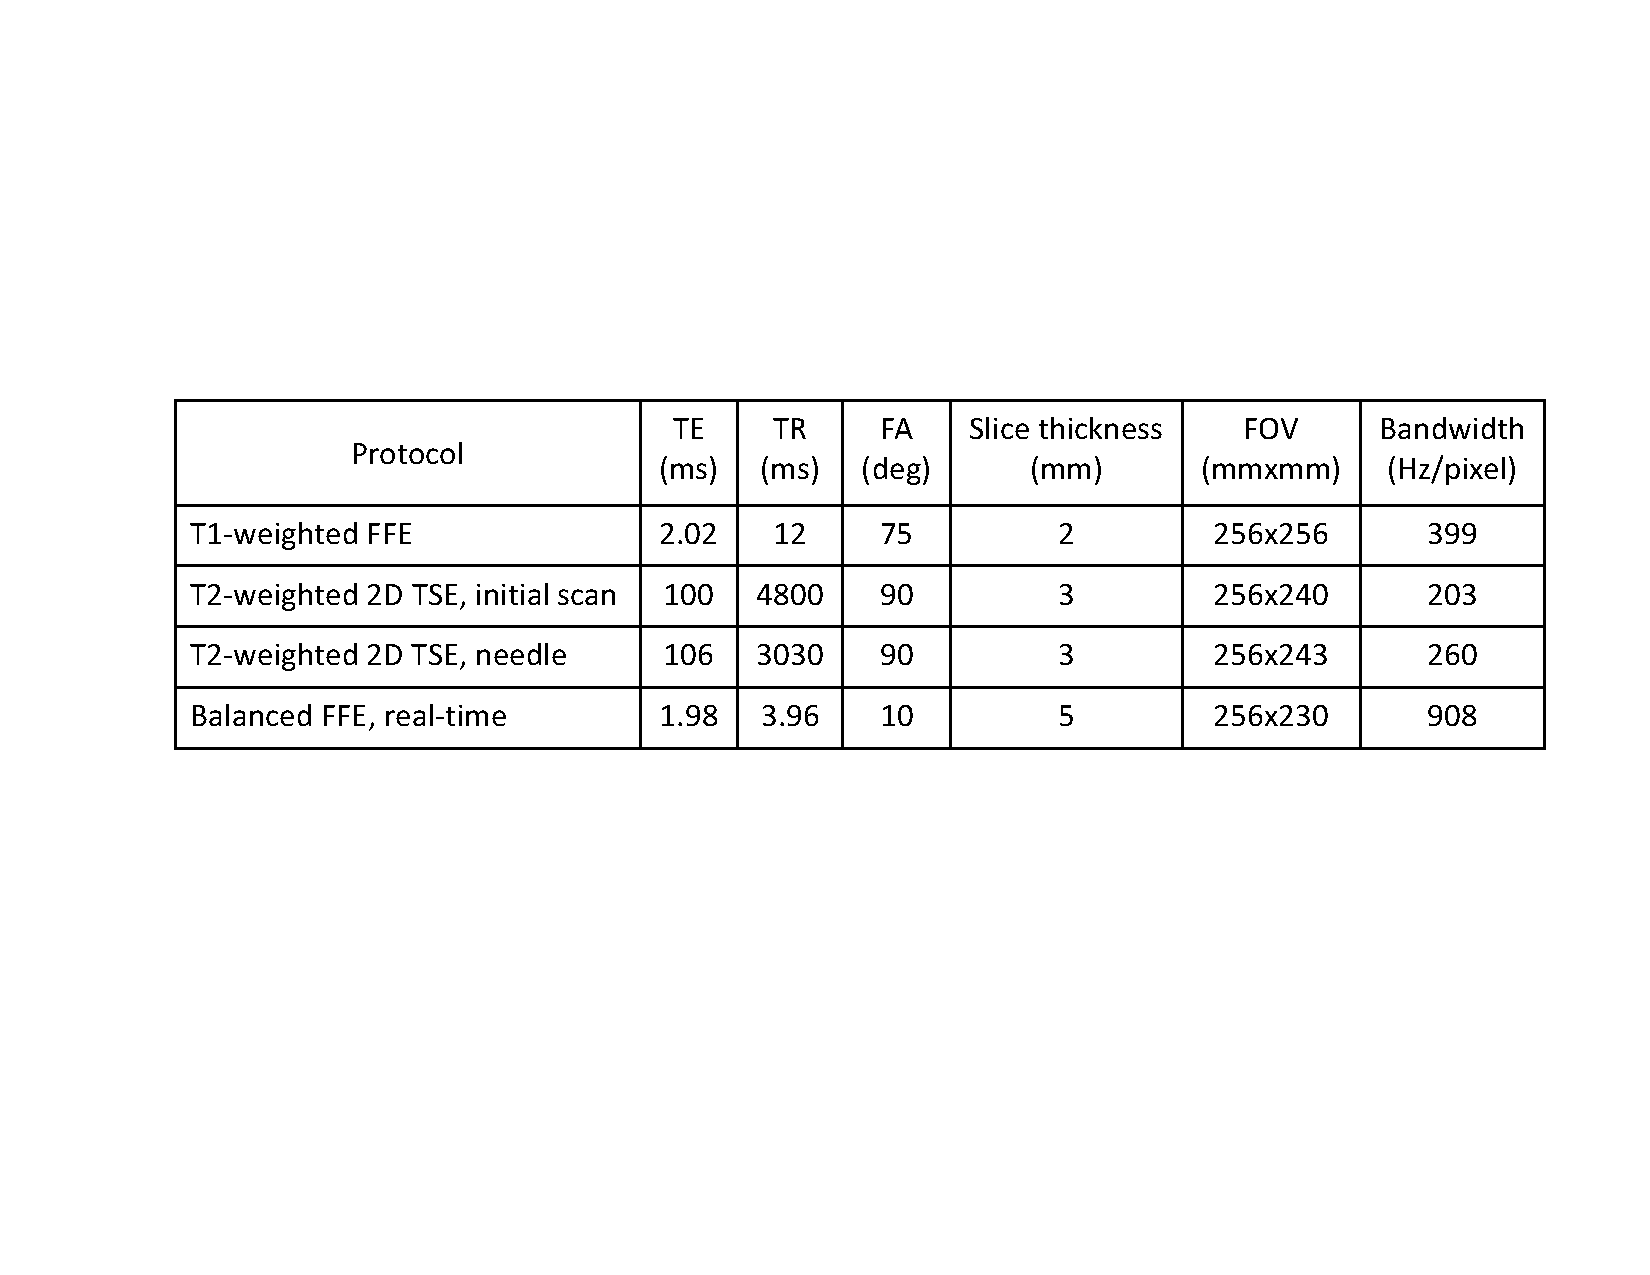
\includegraphics[width=150mm]{Fig/chap1/Protocol.pdf}
% %\caption*{}
% \end{table}
\vspace{-2mm}

% \section{Dissertation Contributions}
% \label{sec:Contributions}

% \begin{itemize}
% \item
% \textbf{Contribution 1}

% Contribution 1

% \item
% \textbf{Contribution 2}

% Contribution 2

% \item
% \textbf{Contribution 3}

% Contribution 3

% \end{itemize}


\section{Thesis Overview}
\label{sec:Overview}
\subsection{Needle Model Integration}
Previous work in needle localization has focused on applying computer vision and image processing algorithms to find the needle tip in camera images and MR data. Particular emphasis has been placed on the calculation of needle positions and orientations for closed-loop control of a robotic insertion system. A useful capability not demonstrated so far would be the use of a mechanical needle model to calculate the expected needle position given the previous needle state and the known inputs at the robot/needle interface, which could be used by the imaging and needle localization systems to improve the imaging rate or measurement accuracy.

\subsubsection{Needle Model Implementation}
The kinematic model proposed by \cite{WebsterModel} has already been implemented and extended by various authors, so it would be a reasonable starting point for needle localization augmentation. I have a working Python implementation of this model.

The addition of torsional dynamics accounting for variable needle depth in the dynamic model shown in \cite{SwensenDynamics} would be useful when working with the thin nitinol needles used to demonstrate small-radius needle steering. The model in \cite{SwensenDynamics} is considerably more technically complex than models in \cite{WebsterModel} or \cite{ReedDynamics}, but I have developed a tentative implementation for an RBE502 Robot Controls project.

Challenges with needle modeling:

- Many models assume that the needle isn't rotated during insertion, and that the deflection is effectively only in one direction.

- Need to represent any conceivable bending configuration

- Limited measurements to fit FEA mode

- Can't measure twist within the needle

\subsection{Improved Needle Localization}

\subsubsection{Needle Localization via Cross-Section}
- Use needle model and bot kinematics to estimate tip depth
- Conduct scan just behind estimated tip position
- Measure actual needle cross section position
- Update model to reflect actual needle behavior
- Reduced dependence on capturing tip in scan plane, less likely to completely lose needle
- Benefits from small FOV
- Use FFE sequence to minimize needle shaft artifact 

\subsubsection{Sizing of Imaging Planes}
The imaging strategy in \cite{AIMNeedleSteering} used conservative imaging parameters to show that closed-loop control of the imaging planes could keep the needle tip within the imaged volume throughout insertion. A comparatively large slice thickness of 10mm was required to guarantee that the imaging planes would never lose tracking during insertion. Extending this system to make model-based predictions of needle behavior would allow the system to move the imaging planes in anticipation of the motion of the needle tip. While the current approach sizes the thickness of the imaging planes to accommodate any possible tip motion between imaging updates, under a model-based approach the slice thickness would be designed around the error between the modeled and actual motion of the needle tip. Under a well-designed model with physically-representative system parameters, this approach would be more accurate than previous efforts. The measured position of the needle tip could update the state of the dynamic model, which would prevent the model from diverging from the actual behavior of the needle during insertion.

\subsection{Alternative Imaging Strategies}
The 2Hz scan rate achieved by \cite{AIMNeedleSteering} represents a baseline and a possible starting point for improvement. The approach used in \cite{AIMNeedleSteering} is to take alternating scans in the coronal and sagittal planes, where the plane of each scan is chosen based on the position of the needle detected in the previous scan in the other plane.  If the position of the needle during insertion is known with some certainty, then a different imaging approach could be used. One option could be to reduce the thickness of the plane, which would improve the visibility of anatomy near the needle but could increase the risk of losing tracking on the needle during insertion.

Another option could be to use a volumetric scan, which would provide voxel data that would determine the 3D needle tip position. A volumetric approach could be more tolerant of off-axis insertion directions, but it would require a significantly different data processing strategy than the current 2D imaging sequence. It might also be too difficult to successfully implement within the scope of this project.

In the context of project work, making modifications to the 2D plane method would be more likely to result in a working system, and the volumetric approach could be researched and implemented later in the project once the capabilities and limitations of the MRI machine and its software are more completely understood.

\subsection{Alternative Scan Plane Orientation}
The coronal/sagittal plane strategy used in \cite{AIMNeedleSteering} assumes that the needle will always be inserted coaxially with the bore of the MRI machine, and that its direction will not significantly deviate during insertion. Modeling of 6-DOF needle pose, coupled with measurement of needle pitch and yaw, would provide sufficient data to realign the scan planes to keep the planes tangential to the tip of the needle. While this would present added complexity in the form of frequently-updated transforms for the scan planes, it could provide better tip localization results, especially if the scan plane is much thinner than the 10mm baseline from \cite{AIMNeedleSteering}.

\subsection{Real-Time Control}
Since real-time needle guidance is the ultimate goal of the project, care should be taken that the chosen implementations do not preclude processing times less than the MRI scan rate. It would also be beneficial to experimental data collection if closed-loop insertion trials could be completed quickly.

\subsection{Slicer Module}
Releasing the above functionality as a Slicer extension would facilitate future research and extension by other groups. The robots used in the AIM Lab are generally designed to communicate via OpenIGTLink, which is already built into Slicer.
- Get more eyes on the research, facilitate transfer to future student

\subsection{Supporting Simulation Software}
The capability to conduct tests independent of the availability of MRI equipment and a suitable insertion platform is highly desirable, especially during the evaluation of steering algorithms. Two pieces of software separate from the Slicer module are required. The first is a kinematic simulator of the insertion robot that can conduct a constant-velocity insertion profile while publishing the pose and velocity of the base of the needle. The second is a simulated MRI scanner, which chooses a volumetric scan from a timestamped series to match the current state of the insertion platform and resections a 2D scan using the field of view and scan plane pose provided by the Slicer module. This combination of utilities will be sufficient to 

% \section{Logistics}
% \subsection{Schedule with Coursework}
% In order to meet the requirements of the thesis-based RBE MS, I will need to complete two more credit-hours of coursework in addition to the nine credit-hours of thesis work. I plan to finish my coursework by taking RBE550 Motion Planning in the Spring semester. I would like to divide research credits approximately equally between the semesters, with five in the Fall and four in the Spring.
% \subsection{Lab Work Hours}
% My experience with my directed research project this past Spring improved my understanding of the extent and distribution of work needed to research, implement, test, and document a component in a robotic system. I initially expected to spend about eight hours per week in the lab, split between Tuesdays and Thursdays, with additional hours to be added as needed. During the week of "crunch time" leading up to the paper submission, I spent about 6 hours per day in the lab, plus extra time during the adjacent weekends. I expect that a consistent 20 hours per week would give enough time to complete the project objectives, with extra time available to conduct experiments using the MRI equipment.
% \subsection{Deadlines and Deliverables}
% A key part of the needle tracking project, and one not present in my initial plan submitted in January, was the push for publication in March. The timeline and work items for my thesis research should be built around known similar goals, and should be sufficiently flexible to accommodate emerging opportunities. It would be reasonable to plan to have the foundational research finished by September and the individual software components prototyped by the end of December 2017, which would leave ample time for iteration and additional development through the end of Spring 2018.

% Marek-motivated papers (Hamlyn, haptics, MRI)

% March IROS journal paper and conference submission deadline

% WPI Master's thesis dissertation paper (this document!)

% Slicer modules: MRI simulation module, needle modeling and tracking module

% Python scripts: stereo needle tip localization and pose estimation

% \subsection{Planned Experiments}
% \subsubsection{Full Phantom Scan Series}
% Insert a needle into the phantom and take full volumetric scans at regular depth intervals. This data will form the basis of the Slicer MRI simulator.

% Does resectioning a volumetric scan in an arbitrary plane produce different results in terms of artifacts, noise, etc than taking a new scan in that plane?
% \subsubsection{MR Needle Tracking Verification}
% Demonstrate tracking by following a needle in real-time in an actual MRI environment. Requires communication of desired scan plane to the MRI machine via its API, which depends on the availability of a compatible MRI machine.
% \subsubsection{CV Tracking Verification}
% Might be a good idea to do the same as above with the stereo needle tracking rig.

% \subsection{Work Items}
% \begin{itemize}
%   \item Learn MRI machine software API and system interface.
%   \item Evaluate practical feasibility of proposed goals, especially volumetric imaging and scan plane rotation.
%   \item Adapt existing needle kinematic and dynamic models to be compatible with needle localization software.
%   \item Devise metrics to show improvement of new tracking algorithm compared to prior efforts.
% \end{itemize}

\section{Methods}



\subsection{Needle Detection}
- Need to sample cross-section points in imagery, to capture needles in "slices".

- Strategy is similar between different imaging modalities.

- In MRI, needle is inserted normal to the axial plane, so the axial slices contain cross-sections of the needle artifact. Threshold each slice to find dark regions, find contours in 2D, and assume that the centroid of the contour closest to the modeled needle is the coordinate of the needle section. Assumes a simplified model for needle artifacts and a limited range of needle insertion trajectories.

- Stereo video is used to track the needle in 3D through transparent tissue phantoms. Emulate behavior of MRI by finding coordinate of needle cross section in a specified plane. Assume needle moves nearly horizontally across camera images. Estimate needle tip coordinate from needle model. Take a column of pixels near the tip coordinate, threshold between light and dark pixels, and find the centroid of the dark region closest to the estimated tip coordinate. Assume that this point lies on the needle shaft. Using matching needle points found in each image, triangulate an estimated 3D point using camera intrinsic and extrinsic parameters. The degree of the polynomial curve fit is a variable that can be adjusted.

- There are two strategies for measuring needle points. We could measure only points close to the tip of the needle. This gives us more updates close to the needle tip, but it assumes that the needle shaft exactly follows the trajectory of the tip, which doesn't hold in soft material. Another option is to resample at different points along the needle shaft. This could present problems in MRI, where each new imaging plane consumes scanning time, but it allows the entire needle model to be updated at once. The frequency of imaging and the spacing between resampling planes are variables.

\subsection{Needle Insertion Platform}
- Used a simple PLA needle guide to center the needle on the phantom during MRI data collection. Plastic spacers on the needle shaft allow the needle base pose to be calculated at each insertion step.

- Used 6-DOF insertion robot during visual needle tracking evaluation. Needle pitch and yaw and translational elements are set before insertion, while needle depth and role are controlled throughout insertion.

\subsection{Software Architecture}
- OpenIGTLink to and from robot, can use Slicer to simulate robot comms

- MRI control via OpenIGTLink. Pick scan planes and field of view.

- INSERT SYSTEM DIAGRAM FIGURE

- Module for real-time needle tracking in MRI.

- Listener registered to volume from MRI, runs segmentation when callback is triggered by update

- Simple ITK used for segmentation, VTK used for homogeneous transforms

\subsection{Experimental Setup}
- MRI data collected for a homogeneous agar gelatin phantom. Needle inserted at regular intervals, full volume collected using XX protocol. Voxel size of 0.4mm x 0.4mm x 0.5mm. Compare estimated tip position from model against manually-labeled tip positions in each volume.

- Stereo vision localization validates real-time approach and communication with robot. Insert needle into homogeneous plastisol phantom with stiffness XX

- Use robotic insertion platform detailed in previous paper [cite Marek]

\section{Results}
- Note: fill in with actual results

\subsection{Stereo Needle Tracking}
- Competing standard would be manually-labeled needle points and tip orientation

- With live tracking, can show that we actually successfully track the needle to a target

- Try for simple case (no rotation) and increasingly rigorous cases (thin needle, many curves, significant deflection)

- Methods to evaluate:

- linear and polynomial regression for all needle points

- Piecewise polynomial minimum bending energy model (3rd and 5th degree)

- Track tip positions vs resample along needle shaft

- Plots: Example insertion for each with curve overlaid. Error for tip pose.

\subsection{MRI Needle Tracking}
- MRI data is limited and very simple: no rotation, deflection in just one direction. Can't do live tracking. Need to show that model accurately finds needle points in each slice and gives a good estimate of the needle tip pose.

- Plots: Curves overlaid on scans.



% \subsection{Timeline (In Development)}
% \begin{tabular}{| l | l|}
%     \hline
%     Date & Milestone \\ \hline
%     2017 \\ \hline
%     September & Foundational Research Finished; Select Needle Dynamic Model \\ \hline
%     October & Demonstrate Existing MRI Tracking System \\ \hline
%     November & Prototype Key Software Components of New Tracking System \\ \hline
    
%     2018 \\ \hline
%     January & Demonstrate New Needle Tracking and Closed-Loop Scan Plane Control \\ \hline
%     February & Data Collection and Design Iteration \\ \hline
%     Mid/Late-March & Prepare Presentation and Documentation \\ \hline
%     Mid-April & Defense \\ \hline
% \end{tabular}

% \section{Conclusion}
% The extension of current research in needle localization and guidance to include model-based estimation of the needle tip during insertion would be of appropriate scope for a MS thesis project.

% \subsection{Goals}
% - Model needle tip pose throughout insertion into a homogeneous medium using the pose of the needle base and the mechanical properties of the needle.
% - Use this pose to choose a MRI scan plane that captures the actual needle position at or very close to the needle tip.
% - Use this measurement to update the needle model and correct for unmodeled deflection.
% - Bundle this functionality as a Slicer module.




% This introductory chapter presents ...

% Chapter 2 introduces ...

% Chapter 3 describes ...

% Chapter 4 presents ...

% Chapter 5 summarizes ...

% Chapter 6 presents ...

% We conclude and discuss future work in Chapter 7. 